\documentclass{scrartcl}
\usepackage{amsmath,amssymb,commath,graphicx,enumerate,listings}
\setkomafont{disposition}{\normalfont\bfseries}

\title{Mat 354}
\subtitle{Homework 5}
\author{Kenny Roffo}
\date{Due October 2, 2015}

\begin{document}
\maketitle

The distribution function is defined $F(y) = P(Y \le y)$

\begin{enumerate}

\item For a random variable $Y$ that is integer valued, $F(12) = 0.2035$ and $F(11) = 0.0658$. Determine $p(y) = P(Y = 12)$.\\
  \begin{align*}
    P(Y = y) &= F(y) - F(y-1)\\
    P(Y = 12) &= F(12) - F(11)\\
              &= 0.2035 - 0.0658\\
              &= 0.1377
  \end{align*}

\item For the case of a simple random sample of 4 integers from $1, 2, ..., 10$ (one of each), and taking $Y$ to be the maximum:\\

  \begin{enumerate}[a)]
    \item Tabulate the distribution function $F(y)$ for values $1, 2, ..., 10$. (If the maximum is no greater than y, then all four values must be no greater than $y$. How many ways can you choose four values no greater than $y$? In how many ways can 4 values be chosen? Divide.)\\

      For a given value $n$, the probability no integer will be greater than $n$ is given by $\frac{n^4}{10^4}$. This $F(Y)$ is given by:
      \begin{center}
        \begin{tabular} { |c|c| }
          \hline
          $Y$&$F(Y)$\\
          \hline
          1  & 0.0001\\
          \hline
          2  & 0.0016\\
          \hline
          3  & 0.0081\\
          \hline
          4  & 0.0256\\
          \hline
          5  & 0.0625\\
          \hline
          6  & 0.1296\\
          \hline
          7  & 0.2401\\
          \hline
          8  & 0.4096\\
          \hline
          9  & 0.6561\\
          \hline
          10 & 1.00000\\
          \hline
        \end{tabular}
      \end{center}
      
    \item Give values for $F(-3), F(0) F(7.5)$ and $F(11.7)$.\\
      \begin{align*}
        F(-3)   &= 0\\
        F(0)    &= 0\\
        F(7.5)  &= 0.2401\\
        F(11.7) &= 1
      \end{align*}

    \item Tabulate the probability function $p(y) = P(Y = y)$ for values $1, 2, ..., 10$. (Use $F$ to help with this. This is the third assignment drilling on this point.)\\
      
      We do this by using $P(Y = y) = F(y) - F(y-1)$:

      \begin{center}
        \begin{tabular} { |c|c| }
          \hline
          $y$&$0(y)$\\
          \hline
          1  & 0.0001\\
          \hline
          2  & 0.0015\\
          \hline
          3  & 0.0075\\
          \hline
          4  & 0.0175\\
          \hline
          5  & 0.0369\\
          \hline
          6  & 0.0671\\
          \hline
          7  & 0.1105\\
          \hline
          8  & 0.1695\\
          \hline
          9  & 0.2465\\
          \hline
          10 & 0.3439\\
          \hline
        \end{tabular}
      \end{center}
\pagebreak
    \item Determine the expected value, variance and standard deviation of $Y$:\\

      \textbf{Expected Value:} For the expected value we use $E(Y) = \sum_{all y}yp(y)$\\
      \begin{align*}
        E(Y) &= 1(0.0001) + 2(0.0015) + 3(0.0075) + ... + 10(0.3439)\\
             &= 8.4667
      \end{align*}\\

      \textbf{Variance:} The Variance is calculated using $E(Y^2) - E(Y)^2$\\
      \begin{align*}
        \sigma^2 &= 1^2(0) + 2^2(0) + 3^2(0) + 4^2(0.00476) + ... + 9^2(0.26667) + 10^2(0.40000) - (8.4667)^2\\
                 &= 2.6167
      \end{align*}

      \textbf{Standard Deviation:} The standard deviation is simply the square root of the variance:\\
      \begin{align*}
        \sigma &= \sqrt{2.6167}\\
               &= 1.6176
      \end{align*}
      
  \end{enumerate}

\item For the case of a random sample (i.e. with replacement) of 4 integers from $1, 2, ..., 10$ (one of each), and taking $Y$ to be the maximum, we found, in class, that $E[Y] = 8.4667$. Suppose we instead sample from $1, 2, ..., k$.:\\
  
  \begin{enumerate}[a)]
  \item Try $k = 5$ and obtain $E[Y]$ numerically. Is $E[Y] = 8.4667/2 = 4.23335$?\\

    Using the same methods as for the previous problem, we obtain a value for $E(Y)=4.4336$ (I am doing these calculations in R in very few lines, so I am not actually seeing the intermediate values, so I don't have them to put in here.). Thus, we cannot scale E(Y) as the amount of numbers change.
    
  \item (You can quickly glean that a simple general expression will not apply by considering $k = 1$.) Challenge? Give a general expression for $E[Y]$ in terms of $k$:\\

    $$\sum_{i=1}^k\left[i\left(\frac{i^4}{k^4} - \frac{(i-1)^4}{k^4}\right)\right]$$

    This was actually pretty easy to come up with considering I had been using it in about three separate steps in R.
  \end{enumerate}
  
\item Suppose $p(y)$ is defined for $y = 1, 2, ..., 9$ (the non-0 digits) as follows: $$p(y) = \log_{10}(y+1) - \log_{10}(y)$$
  \begin{enumerate}[a)]
  \item Construct a table of values $y$ and probabilities $p(y)$. Draw a probability histogram.\\

     \begin{center}
        \begin{tabular} { |c|c| }
          \hline
          $y$&$p(y)$\\
          \hline
          1  & 0.30103\\
          \hline
          2  & 0.1761\\
          \hline
          3  & 0.1249\\
          \hline
          4  & 0.0969\\
          \hline
          5  & 0.0792\\
          \hline
          6  & 0.0669\\
          \hline
          7  & 0.0580\\
          \hline
          8  & 0.0512\\
          \hline
          9  & 0.0458\\
          \hline
        \end{tabular}
      \end{center}

     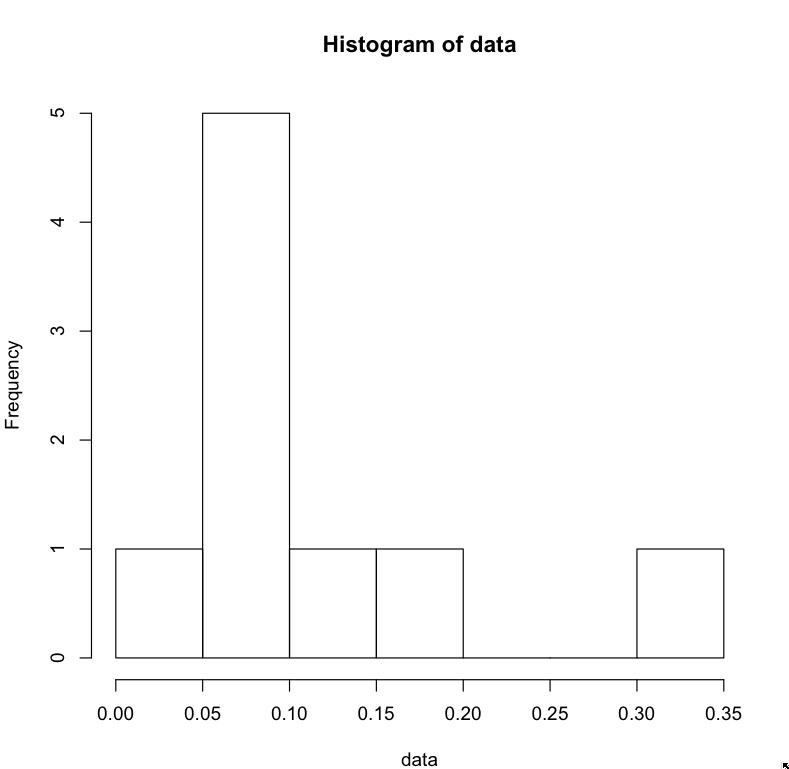
\includegraphics[keepaspectratio=true, scale=0.4]{4a.png}\pagebreak

  \item For a non-zero digit $y$, give the (simplest) formula for $F(y) = P(Y \le y)$.\\
    $$P(Y \le y) = \sum_{i=1}^yp(i)$$

  \item Demonstrate that probabilities given by $p(y)$ sum to exactly 1. That is, show $\sum_{y=1}^9p(y)=1$\\

    Notice that just using the formula we see that many of the logs cancel out, and we are left with $\log(10) - \log(1)$, where $\log(1) = 0$ and $\log(10) = 1$:
    \begin{align*}
      \sum &= \left(\log(2) - \log(1)\right) + \left(\log(3) - \log(2)\right) + ... + \left(\log(10) - \log(9)\right)\\
           &= -\log(1) + \left(\log(2) - \log(2)\right) + ... + \left(\log(9) - \log(9)\right) + \log(10)\\
           &= 0 + 0 + ... + 0 + 1\\
           &= 1
    \end{align*}

  \item Determine $E(Y)$, the expected (or mean) value of $Y$. First obtain a decimal approximation. Then see if you can obtain an exact value (a decimal approximation – no matter how precise – is suboptimal).\\

    Applying $E(Y) = yp(y)$ using the values from part a, we get $E(Y) = 3.440237$.

    Using algebra, we can attempt to find an exact value:
    \begin{align*}
      E(Y) &= \left(\log(2) - \log(1)\right) + 2\left(\log(3) - \log(2)\right) + 3\left(\log(4) - \log(3)\right) + 4\left(\log(5) - \log(4)\right)\\
           &  + 5\left(\log(6) - \log(5)\right) + 6\left(\log(7) - \log(6)\right) + 7\left(\log(8) - \log(7)\right) + 8\left(\log(9) - \log(8)\right)\\
           &  + 9\left(\log(10) - \log(9)\right)\\
           &= -\log(2) - \log(3) - \log(4) - \log(5) - \log(6) - \log(7) - \log(8) - \log(9) + 9\log(10)
    \end{align*}

  \end{enumerate}

\item Wikipedia lists populations of all the “countries” in the world.

You will, for each country, determine the lead digit of the population. For China that digit is 1; for the U.S. that digit is 3. etc.

Download the data set Pops.csv. Read the file into a data frame in R. (Here I’ve used the identifier data for that data frame.) Attach the data frame. You can determine lead digits  using the code that’s supplied. (It’s easier in Excel, where you can use the =LEFT function.)
  \begin{lstlisting}[language=R]
    data <- read.csv([path\_to\_file],header=TRUE)
    attach(data)
    s <- Population/10^floor(log10(Population))
    ld <- floor(s)
  \end{lstlisting}


  \begin{enumerate}[a)]
    \item Obtain a histogram of the Populations. What does this tell you about the populations of countries of the world?\\
      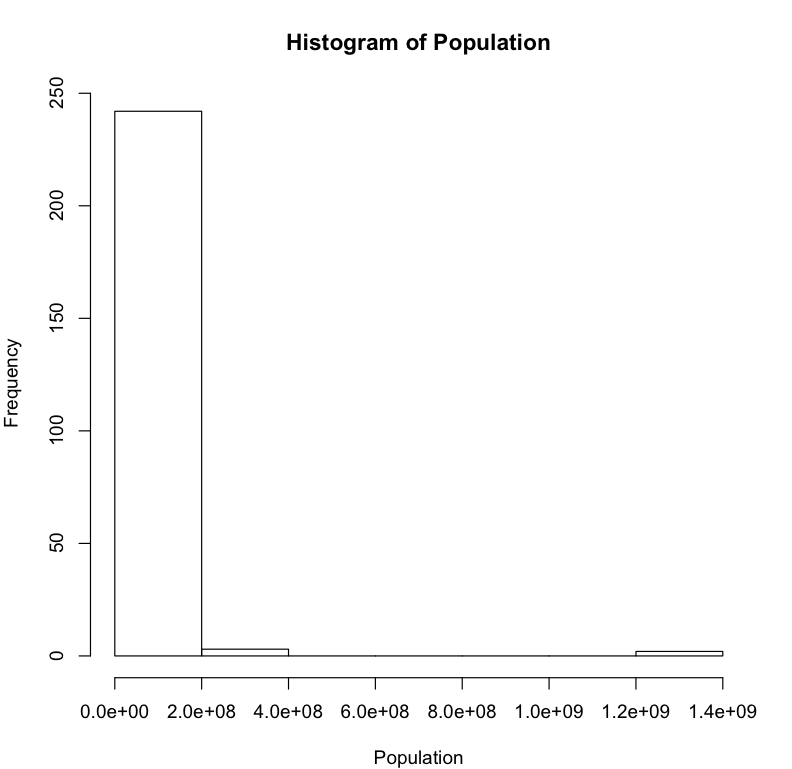
\includegraphics[keepaspectratio=true, scale=0.4]{5a.png}

    \item What’s the population of the world? (You may not be able to use sum directly on the Population variable. I’ll explain later – in class.) To find out, first determine the mean  population of all countries (use mean); then how many (you can use length(Population) to help).\\
      
      7145097761 People

    \item Obtain a histogram of the lead digits.\\
      Left out due to the requirements of part d.

    \item Notice that left to its own devices, R pools all the 1s and 2s. You don’t want to do this. So improve your histogram as follows. Include this histogram only with your assignment.\\

      \begin{lstlisting}[language=R]
        hist(ld, breaks=seq(.5,9.5,1))
      \end{lstlisting}

      \includegraphics[keepaspectratio=true, scale=0.4]{5D.png}

    \item Determine the mean of the lead digits.\\
      3.54251
  \end{enumerate}

\item 
  \begin{itemize}
  \item How does this work?

    \begin{lstlisting}[language=R]
      s <- Population/10^floor(log10(Population))  
      ld <- floor(s)
    \end{lstlisting}

    The right side of the first statement first finds the order (power of 10) each population is, then gets rid of any decimal parts. Then, 10 is raised to this number to give nicely rounded off populations, and the population for the given country is divided by the result to get a number that only has one digit before the decimal. Basically, it just puts a decimal after the first digit of each population. The second statment then floors the results to give only the first digits of all the populations.

  \item What do questions 5 and 6 have to do with each other?\\
    5 is to show how to do something, and 6 is to make sure I understand what's going on.

\end{itemize}
\end{enumerate}

\end{document}

